\begin{figure}[htbp]
\centering
\definecolor{cVer}{HTML}{0072B2}   % verified (computer-algebra) pairs
\definecolor{cRec}{HTML}{D55E00}   % recipe-family prompts D1-D3
\definecolor{cD4}{HTML}{E69F00}    % D4 restatements (unrelated prompt)
\definecolor{cBT}{HTML}{009E73}    % back-translated positives
\definecolor{cMix}{HTML}{CC79A7}   % mixed data, soups, V2 (Section 7)
\definecolor{cMELD}{HTML}{999999}  % MELD-recipe arm
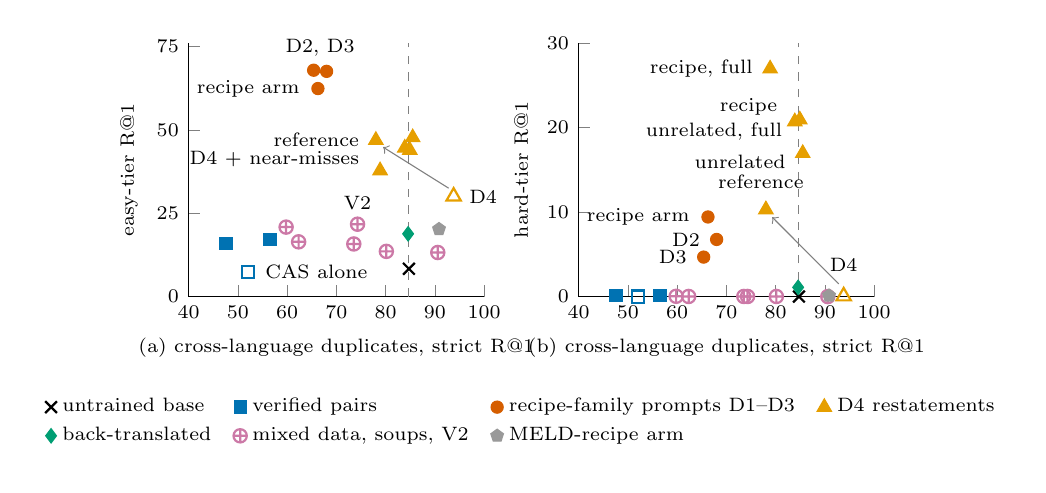
\begin{tikzpicture}
\begin{axis}[
  name=left,
  width=0.44\linewidth, height=4.8cm,
  xmin=40, xmax=100, ymin=0, ymax=76,
  xtick={40,50,60,70,80,90,100}, ytick={0,25,50,75},
  xlabel={(a) cross-language duplicates, strict R@1}, ylabel={easy-tier R@1},
  label style={font=\scriptsize}, tick label style={font=\scriptsize},
  axis y line*=left, axis x line*=bottom, clip=false,
]
\addplot[gray, dashed, forget plot] coordinates {(84.73,0) (84.73,76)};
\addplot[forget plot, only marks, mark=x, mark size=3pt, thick, black] coordinates {(84.73,8.32)};
\addplot[forget plot, only marks, mark=square*, mark size=2.2pt, cVer] coordinates {(56.52,17.05) (47.58,15.92)};
\addplot[forget plot, only marks, mark=square, mark size=2.2pt, thick, cVer] coordinates {(52.08,7.42)};
\addplot[forget plot, only marks, mark=*, mark size=2.2pt, cRec] coordinates {(66.26,62.38) (68.02,67.54) (65.39,67.88)};
\addplot[forget plot, only marks, mark=triangle, mark size=3pt, thick, cD4] coordinates {(93.81,30.03)};
\addplot[forget plot, only marks, mark=triangle*, mark size=3pt, cD4] coordinates {(78.02,46.91) (83.89,44.59) (78.88,37.79) (85.50,47.69) (84.91,43.93)};
\addplot[forget plot, only marks, mark=diamond*, mark size=2.6pt, cBT] coordinates {(84.57,18.81)};
\addplot[forget plot, only marks, mark=oplus, mark size=2.4pt, thick, cMix] coordinates {(74.30,21.70) (59.80,20.83) (80.15,13.55) (73.54,15.77) (62.34,16.41) (90.59,13.21)};
\addplot[forget plot, only marks, mark=pentagon*, mark size=2.4pt, cMELD] coordinates {(90.84,20.23)};
\draw[->, thin, gray] (axis cs:92.8,32.5) -- (axis cs:79.5,44.8);
\node[font=\scriptsize, anchor=east] at (axis cs:64.5,62.38) {recipe arm};
\node[font=\scriptsize, anchor=south] at (axis cs:66.7,69.0) {D2, D3};
\node[font=\scriptsize, anchor=west] at (axis cs:95.0,30.03) {D4};
\node[font=\scriptsize, anchor=east] at (axis cs:76.6,46.91) {reference};
\node[font=\scriptsize, anchor=east] at (axis cs:76.6,41.2) {D4 + near-misses};
\node[font=\scriptsize, anchor=south] at (axis cs:74.30,23.2) {V2};
\node[font=\scriptsize, anchor=west] at (axis cs:53.6,7.42) {CAS alone};
\end{axis}
\begin{axis}[
  name=right,
  at={(left.south east)}, anchor=south west, xshift=1.2cm,
  width=0.44\linewidth, height=4.8cm,
  xmin=40, xmax=100, ymin=0, ymax=30,
  xtick={40,50,60,70,80,90,100}, ytick={0,10,20,30},
  xlabel={(b) cross-language duplicates, strict R@1}, ylabel={hard-tier R@1},
  label style={font=\scriptsize}, tick label style={font=\scriptsize},
  axis y line*=left, axis x line*=bottom, clip=false,
  legend to name=invfulllegend, legend columns=4, legend cell align=left,
  legend style={font=\scriptsize, draw=none, /tikz/every even column/.append style={column sep=6pt}},
]
\addplot[gray, dashed, forget plot] coordinates {(84.73,0) (84.73,30)};
\addplot[only marks, mark=x, mark size=3pt, thick, black] coordinates {(84.73,0.00)};
\addlegendentry{untrained base}
\addplot[only marks, mark=square*, mark size=2.2pt, cVer] coordinates {(56.52,0.16) (47.58,0.16)};
\addlegendentry{verified pairs}
\addplot[forget plot, only marks, mark=square, mark size=2.2pt, thick, cVer] coordinates {(52.08,0.00)};
\addplot[only marks, mark=*, mark size=2.2pt, cRec] coordinates {(66.26,9.42) (68.02,6.76) (65.39,4.67)};
\addlegendentry{recipe-family prompts D1--D3}
\addplot[only marks, mark=triangle*, mark size=3pt, cD4] coordinates {(78.02,10.30) (83.89,20.71) (78.88,26.97) (85.50,16.96) (84.91,20.93)};
\addlegendentry{D4 restatements}
\addplot[forget plot, only marks, mark=triangle, mark size=3pt, thick, cD4] coordinates {(93.81,0.04)};
\addplot[only marks, mark=diamond*, mark size=2.6pt, cBT] coordinates {(84.57,1.09)};
\addlegendentry{back-translated}
\addplot[only marks, mark=oplus, mark size=2.4pt, thick, cMix] coordinates {(74.30,0.01) (59.80,0.03) (80.15,0.01) (73.54,0.01) (62.34,0.01) (90.59,0.00)};
\addlegendentry{mixed data, soups, V2}
\addplot[only marks, mark=pentagon*, mark size=2.4pt, cMELD] coordinates {(90.84,0.11)};
\addlegendentry{MELD-recipe arm}
\draw[->, thin, gray] (axis cs:92.8,1.5) -- (axis cs:79.3,9.4);
\node[font=\scriptsize, anchor=east] at (axis cs:64.5,9.42) {recipe arm};
\node[font=\scriptsize, anchor=east] at (axis cs:66.6,6.76) {D2};
\node[font=\scriptsize, anchor=east] at (axis cs:63.9,4.67) {D3};
\node[font=\scriptsize, anchor=south] at (axis cs:93.81,1.8) {D4};
\node[font=\scriptsize, anchor=south] at (axis cs:77.0,11.6) {reference};
\node[font=\scriptsize, anchor=east] at (axis cs:77.3,26.97) {recipe, full};
\node[font=\scriptsize, anchor=east] at (axis cs:82.3,22.5) {recipe};
\node[font=\scriptsize, anchor=east] at (axis cs:83.3,19.5) {unrelated, full};
\node[font=\scriptsize, anchor=east] at (axis cs:84.0,15.9) {unrelated};
\end{axis}
\node[anchor=north, yshift=-4pt] at (current bounding box.south) {\pgfplotslegendfromname{invfulllegend}};
\end{tikzpicture}
\caption{The full plot behind Figure~\ref{fig:inversion}: every $0.6$B model of Tables~\ref{tab:controlled}, \ref{tab:dose-full}, \ref{tab:factorial} and~\ref{tab:mixing}, with the corrected-gate retrains and V2's no-instruction reading omitted. Same axes and conventions as Figure~\ref{fig:inversion}: horizontal, strict R@1 on cross-language duplicates, the dashed line and $\times$ the untrained base; colour, what the positives are; hollow, no negatives; the labels on the D4 cells name the negatives attached (``recipe'' and ``unrelated'' are LLM near-misses from the recipe's prompt and from an unrelated one, ``full'' at the recipe arm's negative volume). Two groups appear here only: the verified squares also include computer-algebra positives with no negatives (CAS alone) and the uncapped verified arm, and the crossed circles are the mixed-data, soup and V2 models of Appendix~\ref{sec:forgetting}, which sit near the hard-tier floor. The MELD-recipe arm is seed $42$ ($20.23$ easy, $0.11$ hard, $90.84$ real; Section~\ref{sec:ood}). (a)~Easy tier: every model trained on LLM rewrites scores above the verified ones. (b)~Hard tier: only deep LLM rewrites paired with negatives reach it; the arrow is the edit from D4 alone to the reference, attaching verified negatives, which lifts hard R@1 off the floor and costs $15.79$ retention points, and LLM-written near-misses lift the same restatements further (Table~\ref{tab:factorial}). Computer-algebra positives with the recipe's near-misses lie off the axis at $12.47$ real.}
\label{fig:inversion-full}
\end{figure}
